In this chapter, we lay the groundwork for the research conducted in this thesis by presenting an overview of the fundamental concepts and algorithms related to the \mst\ problem. We begin with a detailed examination of classical \mst\ algorithms including {\tt Prim}'s algorithm, {\tt Kruskal}'s algorithm—along with its associated {\tt Union-Find} data structure—and {\tt Boruvka}'s algorithm. Following this, we explore parallel and distributed approaches to the \mst\ problem, providing a general overview before delving into specific methods such as the \FKruskal\ algorithm and the Message Passing {\tt Prim} algorithm.

The chapter also covers the topic of fully dynamic {\mst}s, discussing both sequential and parallel/distributed approaches, most of them theoretical since there is little work in experimental. Finally, we introduce the Dynamic Pipeline Approach, setting the stage for its application in solving the \mst\ problem, which will be further elaborated in the subsequent chapters. This comprehensive review equips the reader with the necessary background to understand the innovations and experimental analyses presented later in the thesis.

\section{Minimum Spanning Tree}

\begin{definition} \label{def:graph}
A \textit{graph} $G$ consists of two sets: a set of vertices $V$ and a set of edges $E$, where $E$ is a set of unordered 
pairs from $V$ such that $E \subseteq \{\{u,v\}\,|\,u,v\in V\}$. $G$ is usually denoted as $G=(V,E)$. 
\end{definition}

From now on, unless stated otherwise, for any graph $G=(V,E)$, we will refer to the elements of $V$ indistinctly as the vertices or the nodes of $G$ and to its size as $n$ ($|V| = n$). 
Likewise we will refer to the elements of $E$ as the set of edges of $G$ and we will say that the size of $E$ is $m$ ($|E| = m$). 


\begin{definition} \label{def:wgraph}
A \textit{weighted graph} $G= (V,E)$ is a graph in which its edges are assigned numerical values (known as weights) given by a function $\omega: E \rightarrow \mathbb{R}^+$.
\end{definition}

An example of a weighted graph is shown in Figure~\ref{fig:example_graph}. 

\begin{definition} \label{def:st}
A \textit{spanning tree $T$ of a graph $G$} is a subgraph of $G$ that is a tree and includes all the vertices of $G$. 
\end{definition}

For the purposes of our work, if a graph $G$ is not connected, we will work with its \textit{spanning forest}. 
A spanning forest of a graph $G$ is a subset $F$ of $G$ conformed by a set of trees such that for every connected component 
of $G$, exactly one spanning tree of the connected component is in $F$.
From now on,  abusing of notation, we will refer to a spanning forest of a non connected graph $G$ as a spanning tree of $G$. 
Figure \ref{fig:example_spanning} shows a spanning tree of the graph of Figure~\ref{fig:example_graph}. 
The light-gray dashed edges have not been added to the spanning tree.

\begin{figure}
    \centering
    \begin{subfigure}{0.48\textwidth}
        \tikzstyle{new style 0}=[fill=white, draw=black, shape=circle, align=center]
\tikzstyle{tree_edge}=[-, draw=black]

\begin{tikzpicture}
	\begin{pgfonlayer}{nodelayer}
		\node [style=new style 0] (0) at (-4, 2.65) {a};
		\node [style=new style 0] (1) at (-4, 0) {b};
		\node [style=new style 0] (2) at (-1, 2.65) {c};
		\node [style=new style 0] (3) at (-1, -2.65) {d};
		\node [style=new style 0] (4) at (-7, 2.65) {e};
		\node [style=new style 0] (5) at (-7, -2.65) {f};
		\node [style=new style 0] (6) at (-4, -2.65) {g};
	\end{pgfonlayer}
	\begin{pgfonlayer}{edgelayer}
		\draw [style={tree_edge}] (0) to["1"] (1);
		\draw [style={tree_edge}] (1) to["0.3"] (2);
		\draw [style={tree_edge}] (2) to["2.5"] (0);
		\draw [style={tree_edge}] (2) to["10"] (3);
		\draw [style={tree_edge}] (0) to["2"] (4);
		\draw [style={tree_edge}] (1) to["1.5"] (5);
		\draw [style={tree_edge}] (5) to["5.57"] (6);
		\draw [style={tree_edge}] (1) to["0.05"] (6);
	\end{pgfonlayer}
\end{tikzpicture}
        \caption{A weighted graph.}
        \label{fig:example_graph}
    \end{subfigure}
    \begin{subfigure}{0.48\textwidth}
        \tikzstyle{new style 0}=[fill=white, draw=black, shape=circle, align=center]
\tikzstyle{separator}=[-, dashed, draw=lightgray]
\tikzstyle{tree_edge}=[-, draw=black]

\begin{tikzpicture}
	\begin{pgfonlayer}{nodelayer}
		\node [style=new style 0] (0) at (-4, 2.65) {a};
		\node [style=new style 0] (1) at (-4, 0) {b};
		\node [style=new style 0] (2) at (-1, 2.65) {c};
		\node [style=new style 0] (3) at (-1, -2.65) {d};
		\node [style=new style 0] (4) at (-7, 2.65) {e};
		\node [style=new style 0] (5) at (-7, -2.65) {f};
		\node [style=new style 0] (6) at (-4, -2.65) {g};
	\end{pgfonlayer}
	\begin{pgfonlayer}{edgelayer}
		\draw [style={tree_edge}] (0) to["1"] (1);
		\draw [style={tree_edge}] (1) to["0.3"] (2);
		\draw [style={separator}] (2) to["2.5",text=lightgray] (0);
		\draw [style={tree_edge}] (2) to["10"] (3);
		\draw [style={tree_edge}] (0) to["2"] (4);
		\draw [style={tree_edge}] (1) to["1.5"] (5);
		\draw [style={separator}] (5) to["5.57",text=lightgray] (6);
		\draw [style={tree_edge}] (1) to["0.05"] (6);
	\end{pgfonlayer}
\end{tikzpicture}

        \caption{A spanning tree.}
        \label{fig:example_spanning}
    \end{subfigure}
    \caption{An example of a weighted graph and one of its spanning trees}
\end{figure}

%\begin{definition} \label{def:mst}
%Given a weighted graph $G=(V,E)$, with $\omega: E\rightarrow \mathbb{R}^+$ and a spanning tree $T=(V,E')$ of $G$, $T$ is a \textit{minimum spanning tree of $G$} ( \mst) iff for all spanning tree $T'$ of $G$, $T'=(V,E'')$ and $T'\neq T$,  $ \sum_{e\in E'} \omega(e) \leq \sum_{e\in E''} \omega(e)$.
%\end{definition} 

\begin{definition}\cite{AlgorithmicsNotes} 
\label{def:mst}
Given a weighted graph $G=(V,E)$, $\omega: E\rightarrow \mathbb{R}^+$, we say that $T=(V,E')$, with $E' \subseteq E$, is a \textit{minimum spanning tree} of $G$ if $T$ is a spanning tree of $G$ that minimizes:
\[
\omega(T) = \sum_{e \in E'} \omega(e)
\]
\end{definition}
Let us observe that the spanning tree shown in Figure \ref{fig:example_spanning} is a minimum spanning tree of the graph shown therein.

From now on, abusing of notation, as long as it does not generate ambiguities and unless stated differently, we will use \mst\ as an abbreviation of minimum spanning tree and \mst(G) as the minimum spanning tree of graph $G$.

The finding and computation of \msts\ remains as a common challenge in graph theory, leading to the development of various algorithms to address it. Notable among these are Prim's~\cite{Prim1957}, Kruskal's~\cite{Kruskal1956}, and Bor\r{u}vka's~\cite{Boruvka1926} algorithms, each leveraging different useful properties of \msts. These algorithms will be succinctly discussed in the subsequent subsections.

\msts\ have some useful properties: the cut-property and the cycle-property~\cite{TarjanDSandNA}. A \textit{cut} is a partition of the vertices of a graph into two disjoint subsets. The \textit{cut-set} of a cut is the set of edges that have one endpoint in each subset of the partition. The cut-property states that for any cut $C$ of the graph, if the weight of an edge $e$ in the cut-set of $C$ is strictly smaller than the weights of all other edges of the cut-set of $C$, then this edge belongs to all \msts\ of the graph. A \textit{cycle} is a finite sequence of edge which joins a sequence of vertices in which only the first and last vertices are equal. The cycle-property states that for any cycle $C$ in the graph, if the weight of an edge $e$ of $C$ is larger than any of the individual weights of all other edges of $C$, then this edge cannot belong to an \mst.

\subsection*{Prim's Algorithm \label{sec:prim}}

{\tt Prim}'s Algorithm separtes the vertices in two subsets, those already added to the \mst\ and those that are not added yet. It starts adding any given vertex to the \mst. Then, in every iteration, it chooses the lightest edge that connects the vertices in the \mst\ with the vertices not added yet and repeats until all the vertices are added. Algorithm \ref{alg:prim} shows a sketch in pseudo-code adapted from~\cite{TarjanDSandNA}. Prim's algorithm implemented as described has a running time of $O(n^2)$, but can be reduced up to $O(m \frac{\log n}{\log{(2 + m/n)}})$~\cite{TarjanDSandNA}.

\begin{algorithm}[H]
\caption{Prim's algorithm \label{alg:prim}}
\begin{algorithmic}
    \Procedure{Prim}{$G$}
        \State $u \gets \text{Select one of }V(G)$
        \State $F \gets \varnothing$
        \State $Q \gets V(G) \setminus \{u\}$
        \State $V(F) \gets \{u\}$
        \While{$Q \neq \varnothing$}
            \State $e \gets \argmin_{\{e=\{u,v\} \in E(G)  | u \in V(F) \land v \in Q \}} \omega(e)$
            \State $Q \gets Q \setminus \{ v \}$
            \State $F \gets F \cup \{e\}$
        \EndWhile
        \State \Return $F$
    \EndProcedure
\end{algorithmic}
\end{algorithm}


\subsection*{Kruskal's Algorithm\label{sec:mst:kruskal}}
This algorithm uses the cycle property of \msts. 

The idea behind the algorithm is the following: in every iteration add the lightest edge to the forest unless it forms a cycle - which happens when two vertices belong to the same connected component, $CC$. Algorithm \ref{alg:kruskal} shows a sketch in pseudo-code adapted from~\cite{TarjanDSandNA}. The sorting step requires $O(m \log n)$ time and the time for the connected components is $O(m \alpha(m,n))$. The function $\alpha(m,n)$ is the inverse Ackermann function which grows much slower than the logarithm function and usually it is considered constant since $\alpha(n)$ is less than 5 for any practical input size $n$. Thus the total running time is $O(m \log n)$~\cite{TarjanDSandNA}.

\begin{algorithm}[H]
\caption{Kruskal's algorithm \label{alg:kruskal}}
\begin{algorithmic}
    \Require $E$ to be in weight-ascending order
    \Procedure{Kruskal}{$G = (V,E)$}
        \State $F \gets (V, E' = \varnothing)$
        \For{$e=(u,v) \in E$}
            \If{$CC_F(u) \neq CC_F(v)$} \Comment{$CC_F(u)$, the connected component of $u$ in $F$}
                \State $F \gets (V, E' \cup \{e\})$
            \EndIf
            %\If{Sets.\Call{FindSet}{$u$} $\neq$ Sets.\Call{FindSet}{$v$}}
            %    \State $F \gets F \cup \{e\}$
            %    \State Sets.\Call{Union}{$u, v$}
            %\EndIf
        \EndFor            
        \State \Return $F$
    \EndProcedure
\end{algorithmic}
\end{algorithm}

\subsection*{Bor\r{u}vka's Algorithm}
This algorithms uses two properties of the \msts: the cut property already explained and the contraction property. The contraction property states that iff $T$ is a tree of \mst\ edges, then we can contract $T$ into a single vertex while maintaining the invariant that the \mst\ of the contracted graph plus $T$ gives the \mst\ for the graph before contraction.

The idea behind this algorithm is that initially the \mst\ is empty and every vertex is single component in the \mst. Then, in every iteration for every component, the cheapest edge that connects it to some other component is found and added to the \mst. Algorithm \ref{alg:boruvka} shows a sketch in pseudo-code adapted from~\cite{TarjanDSandNA}. Each iteration can be done in $O(\log n)$ and there is at most $m$ iterations, thus the total running time is $O(m \log n)$~\cite{TarjanDSandNA}.

\begin{algorithm}
\caption{Bor\r{u}vka's algorithm \label{alg:boruvka}}
\begin{algorithmic}
    \Procedure{Bor\r{u}vka}{$G = (V,E)$}
        \State $F \gets (V, E' = \varnothing)$
        \State $Completed \gets \texttt{False}$
        \While{$\neg Completed$}
            \State Find the connected components (CC) of $F$
            \State Initialize the cheapest edge for each component to $\varnothing$
            \For{ $e = \{u,v\} \in E, CC(u) \neq CC(v)$}
                \State $e' \gets cheapest\_edge(CC(u))$
                \If{$\omega(e) < \omega(e')$}
                    \State $cheapest\_edge(CC(u)) \gets e$
                \EndIf
                \State $e' \gets cheapest\_edge(CC(v))$
                \If{$\omega(e) < \omega(e')$}
                    \State $cheapest\_edge(CC(v)) \gets e$
                \EndIf
            \EndFor
            \State $Completed \gets \texttt{True}$
            \For{ $i \in CC$}
                \State $e \gets cheapest\_edge(i)$
                \If{$e \neq \varnothing$}
                    \State $F \gets (V, E' \cup \{e\})$
                    \State $Completed \gets \texttt{False}$
                \EndIf
            \EndFor
        \EndWhile
        \State \Return $F$
    \EndProcedure
\end{algorithmic}
\end{algorithm}


\subsection*{Parallel and/or Distributed Algorithms}
The problem of computing the \mst\ of a connected graph has also been studied 
for parallel and concurrent models of computation leading 
to several algorithms~\cite{bader2006fast,durbhakula2020parallel,tripathy2013new}. 

In the parallel model the objective is to minimize the maximum number of steps of 
computation that are performed by each processor as well as the number of processors involved, 
while in the distributed model the objective is to minimize the number of rounds of communication 
between the processors that are supposed to be of unbounded computational power. 
Also the algorithms in the parallel case assume that the processors have shared memory 
and this is not the case in distributed model.
In particular, Bader et al.~\cite{bader2006fast} implement three parallel 
variants of Bor\r{u}vka's \mst\ algorithm~\cite{chung1996parallel} arguing that 
this algorithm is more naturally paralelizable than Prim's and Kruskal's ones. 
The authors in~\cite{bader2006fast} claim that --by the first time-- they 
present a general parallel \mst\ algorithm that runs efficiently in the 
SMP computer architecture\footnote{SMP computer architecture is a multiprocessor hardware and software architecture that has multiple identical processors. 
Processors share main memory and have access to all I/O devices.}. In the distributed
memory model such as the BMP computer architectue~\cite{Valiant1990}, the authors in~\cite{Lonar2014}
provide working an experimental comparison of algorithms based on Prim and Kruskal.

Independently of the topology of the input graphs, all these algorithms 
are designed for working on \textit{in-memory} and/or static graphs --contrary to dynamic ones. 
To overcome the memory-bound problem, \mst\ distributed algorithms 
have been proposed~\cite{pandurangan2018distributed} where 
it is necessary to deal with  message passing overhead, 
memory latency and fault-tolerance issues~\cite{burkhardt2015cloud}.

\subsubsection{Filter Kruskal \label{sec:filter_kruskal}}

\FKruskal\ is a divide-and-conquer variant of Kruskal's algorithm inspired by the principles of Merge Sort~\cite{Osipov2009}. This algorithm effectively partitions the graph's edges to facilitate parallel processing. The main idea is to choose a pivot edge, then separate the remaining edges into two subsets: those with weights less than the pivot and those with weights greater than the pivot. The algorithm recursively processes the lower-weight subset to build a partial \mst. For the higher-weight subset, it removes edges that do not contribute to the \mst\ (i.e., edges that connect vertices already in the same component). This approach leverages parallelism by dividing the problem into smaller, independent subproblems.

The \FKruskal\ algorithm is particularly advantageous for its simplicity in parallelization, as noted by its authors~\cite{Osipov2009} and has an expected running time of $O(m + n \log (n) \log (m/n))$. Below is the detailed pseudocode:

\begin{algorithm}[H]
\caption{Filter Kruskal's algorithm \label{alg:fkruskal}}
\begin{algorithmic}
    \Procedure{\FKruskal}{$G=(V,E)$}
        \If{$|E| < $ threshold}
            \State \Return \Call{Kruskal}{$G$}
        \Else
            \State $p \gets $ pivot in $E$
            \State $E_{\le} \gets \{e \in E : \omega(e) \le \omega(p) \}$
            \State $T_{\le} = (V,E'_{\le}) \gets\ $\Call{\FKruskal}{$(V, E_{\le})$}
            \State $E_{>} \gets \{e=(u,v) \in E : \omega(e) > \omega(p)\ \land\ CC_T(u) \neq CC_T(v)\}$
            \State $T_{>} = (V,E'_{>}) \gets\ $\Call{\FKruskal}{$(V, E_{>})$}
            \State \Return $(V, E'_{\le} \cup E'_{v})$
        \EndIf
    \EndProcedure
\end{algorithmic}
\end{algorithm}

In this algorithm, if the number of edges $|E|$ is below a certain threshold, the algorithm switches to the standard Kruskal's algorithm for simplicity and efficiency. A pivot edge $p$ is selected from the graph $G$. This pivot helps in dividing the graph's edges into two subsets. The subset of edges $E_{\le}$ containing edges with weights less or equal than $p$ is recursively processed to build the \mst. For the subset of edges $E_{>}$ with weights greater than $p$, edges that do not contribute to the \mst\ (those connecting vertices already in the same component) are filtered out. The remaining edges are recursively processed.

This approach not only ensures the correctness of the \mst\ but also enhances efficiency by leveraging parallel processing, making it suitable for large-scale dynamic graphs. 

\subsubsection{Parallel Prim \label{sec:parallel_prim}}
Lončar et al.~\cite{Lonar2014} provide a parallelization of Prim algorithm (basic algorithm explained in Section~\ref{alg:prim}). Only two steps can be parallelized: selection of the minimum-weight edge connecting a vertex not in \mst\ to a vertex in \mst, and updating array $d$ -an auxiliary array of length $n$ to store distances from each vertex to \mst- after a vertex is added to \mst.

The algorithm partitions the input set $V$ into $k$ subsets, where each subset contains $n/k$ 
consecutive vertices along with their associated edges. Each process is assigned a distinct subset. In addition to their vertex subsets, each process also manages a portion of the array $d$, which tracks distances for the vertices in its partition. Let $V_i$ represent the subset assigned to process $p_i$, and $d_i$ the corresponding segment of the array $d$ that $p_i$ maintains.

Each process $p_i$ identifies the minimum-weight edge $e_i$ (the candidate edge) that connects a vertex in the \mst\ to a vertex in $V_i$. These candidate edges are then sent from each process $p_i$ to the root process using an all-to-one reduction. The root process selects the edge with the minimum weight from the received candidates, adds this edge to the \mst, and broadcasts the selected edge to all other processes. Each process then updates its local portion of the array $d$ and marks the vertices connected by this edge as part of the \mst.

This process is repeated iteratively until every vertex is included in the \mst.

Finding a minimum-weight edge and updating $d_i$ during each iteration costs $O(p/n)$. Each step also performs a communication between the processes which takes $O(\log p)$. Combining the cost of one iteration and since there are $n$ iterations, the total parallel time is: $O(n^2/p + n\log p)$.

\section{Algorithms for Fully Dynamic \mst}

A static weighted graph according to Definition~\ref{def:wgraph} involves a set of nodes $V$, a set of edges $E$, and a weight function $\omega$. A weighted \emph{dynamic graph} is obtained when any of these four entities changes over time~\cite{Harary1997}. A dynamic graph allows three kind of operations: insert a new edge, delete an edge of the graph and update the weight of an edge. If only one of this operations is allowed, we say that it is a \emph{Partially Dynamic Graph}. On the other hand, if any operation is allowed, it is a \emph{Fully Dynamic Graph}. We call any instance of these operations an \emph{event}: 
\begin{enumerate}[(i)]
\item {\label{op:update} {\opupdate$(G,e,\omega_e)$} where the previous 
weight of edge $e\in E$ is replaced by $w_e$}
\item {\label{op:insert} {\opinsert$(G,e,\omega_e)$} that inserts edge $e$ in $E$ 
and assigns to it weight $\omega_e$ }
\item {\label{op:remove} {\opremove$(G,e)$} that removes $e$ from $E$.}
\end{enumerate}

The study of dynamic graphs and, in particular, of algorithms that maintain a \mst of the dynamic
graph is not new. In the extensive survey of Hanauer, Henzinger and Schulz~\cite{Hanauer2022}
there is a reasoned state of the art on these algorithms that divides them 
clearly into theoretic algorithms and practical ones. Regarding specifically the
maintenance of the \mst\ of dynamic graphs, there has been very little work done
on both theoretical algorithms and their empirical evaluation. 

Frederickson~\cite{Frederickson1985} proposed a data structure for online updating
of \mst\ with a cost of $O(\sqrt{m})$ per update. Their proposal uses as base a 
previous work by Sleator and Tarjan~\cite{Sleator1983} for 
maintaining a dynamic tree. Frederickson's solution applies a preprocessing step 
that forces all the graphs to have degree at most 3, by adding new vertices that 
are connected with weight zero. Holm et al.~\cite{Holm2001} gave the first 
fully dynamic algorithm with poly-logarithmic time per operation improving it 
later to $O(\log^4 n/\log\log n)$ amortised time per operation~\cite{holmetal2015}.
The lower bound of $\Omega(\log n)$ per operation on graphs of $n$ vertices for 
connectivity of dynamic graphs was extended by Patrascu et al.
~\cite{Patrascu2006} to maintaining \msts.

On the empirical evaluation, we can find the work of Amato~\cite{Amato1997} or
Cattaneo et al.~\cite{cattaneo2010} that provide an extensive experimental study
that assesses different approaches: 

\begin{enumerate}[a)]
    \item Eppstein et al.'s sparsification~\cite{eppstein1997sparsification,eppstein1998separator,eppstein1992maintenance}
    \item Frederickson's partitions and topology trees~\cite{Frederickson1985,frederickson1997ambivalent}
    \item Holm et al.'s logarithmic decomposition~\cite{holmetal2015}
\end{enumerate}

The experiments therein~\cite{cattaneo2010} have shown that, except for very 
particular instances, a simple $O(m \log n)$-time algorithm has the best 
performance in practice (for graphs of $n$ vertices and $m$ edges) and
runs substantially faster than the poly-logarithmic algorithm of Holm et al.~\cite{holmetal2015}: 
the latter was faster than the first for only one out of five different
classes of instances, namely those in $k$-clique graphs, in which small cliques are
connected by some inter-clique edges and all updates involve only the inter-clique edges. 
Despite its good theoretical amortized running time, the complex chain of data structures 
supporting Holms et al.~\cite{holmetal2015} algorithm does not seem to lead to fast implementations 
and may require too much memory. 

For the specific case of graphs with changing weights --i.e. the edges of the graph are
constant, but the edge weights can change dynamically--  Ribero and 
Toso~\cite{Ribeiro2007} proposed a $O(m)$ amortized running time algorithm 
--for graphs of $m$ edges-- that reduces the computation time observed for the 
algorithm of Cattaneo et al.~\cite{cattaneo2010}, yielding the fastest experimental
algorithm for the above mentioned graphs.

Up to our knowledge, the only parallel and /or distributed algorithm dealing with the 
maintenance of the \mst\ of fully dynamic graphs was given by Nowicki~\cite{nowicki2021dynamic}. 
The algorithm is based on the massively parallel computation (MPC) computation model 
(MapReduce)~\cite{Karloff2010}, but it is restricted to sequences of updates of 
sub-linear size (with respect to the graph size).

\section{Dynamic Pipeline}
Big data and the Internet of Things (IoT) are pivotal in driving both industrial
digitization and interdisciplinary scientific research. Data-driven frameworks, 
which adapt execution schedulers and computational structures to current input 
data conditions, are essential for managing continuous data streams. Data 
Streaming (DS) has been approached through various methods to efficiently process
large volumes of data with high parallelization. Two distinct parallelization 
models have been identified: Data Parallelism (DAP) and Pipeline Parallelism (PP).
Data-driven frameworks, which adapt execution schedulers and computational 
structures to current input data conditions, are essential for managing continuous
data streams. However, traditional parallel paradigms like 
MapReduce~\cite{Dean2008,Karloff2010}, which rely on the Divide \& Conquer 
approach, have limitations. They partition problems into subproblems that must be
fully executed before proceeding, resulting in a blocking behavior that impedes 
incremental result generation and limits the flexibility needed for real-world 
applications. In contrast, the Dynamic Pipeline Approach~\cite{Zoltan2019,Pasarella2024}
(\dpm) is a PP computational model that operates as a one-dimensional, 
unidirectional chain of stages implemented as an asynchronous model of computation
synchronized by channels, enabling the simultaneous execution of dependent tasks
on different data items.

In the \dpm\, stages can be categorized into several types: input stages, filter stages, generator stages, and output stages. Input stages are responsible for reading and feeding data into the pipeline. Filter stages process the data, applying transformations or filtering operations as needed. Generator stages can produce new filter stages based on the current data flow. Finally, output stages handle the end result, such as writing data to storage or presenting it to the user. Modeling a problem within the \dpm\ involves breaking it down into filters. For example, a graph-processing problem can be approached by having filter stages apply partitioning to the graph and algorithms to process the vertices and edges, ensuring that the solution can be built incrementally from the output of the previous filter.

Many different problems have been implemented in the \dpm, see Figure~\ref{fig:examples_dp}. Authors in~\cite{Pasarella2017} use DP for the well-known problem of counting 
triangles in a graph. Results suggest that pipeline allows for the implementation 
of an efficient solution of the problem of counting triangles in a graph, 
particularly, in dense and large graphs, drastically reducing the execution time 
with respect to the MapReduce implementation. The problem of enumerating bitriangles
in large bipartite nerworks~\cite{Royo_Sales_2021,Royo2021} have also been 
implemented efficiently in the \dpm. Another example of problems solved in \dpm\ is 
given in~\cite{Lugosi_Enes_2019}. In this work, authors propose a 
working implementation for solving the problem of multidimensional range queries, 
the retrieval of points of a multidimensional space that fall inside a given region.

\begin{figure}
    \centering
    \begin{subfigure}{\textwidth}
    \centering
        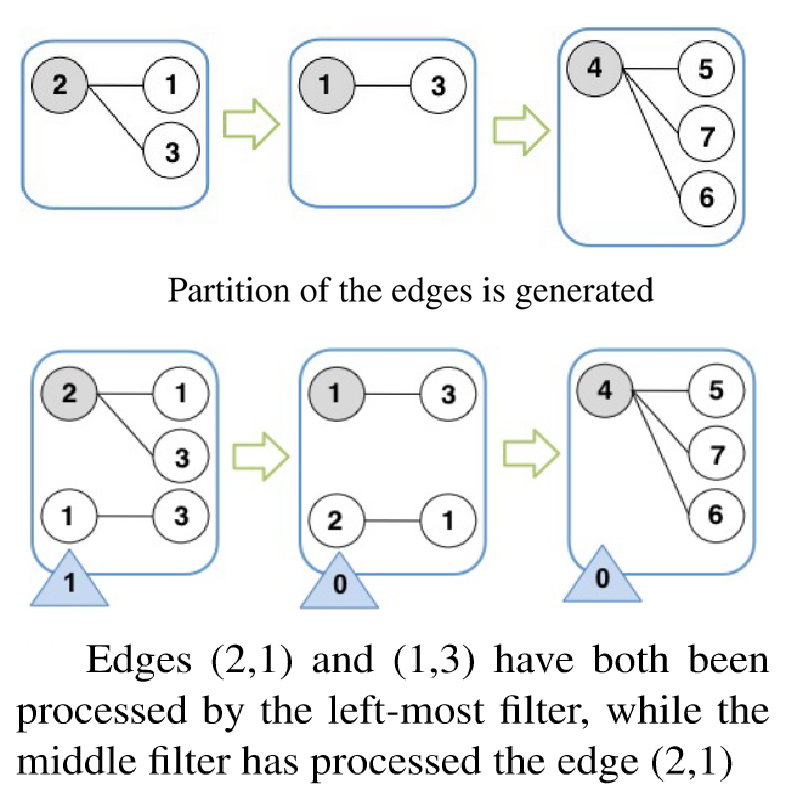
\includegraphics[width=0.5\textwidth]{figures/ExampleTriangles.png}
        \caption{Dynamic Pipeline for triangles in graphs. Images from \cite{Pasarella2017}}
    \end{subfigure}
    \hfill
    \begin{subfigure}{\textwidth}
    \centering
        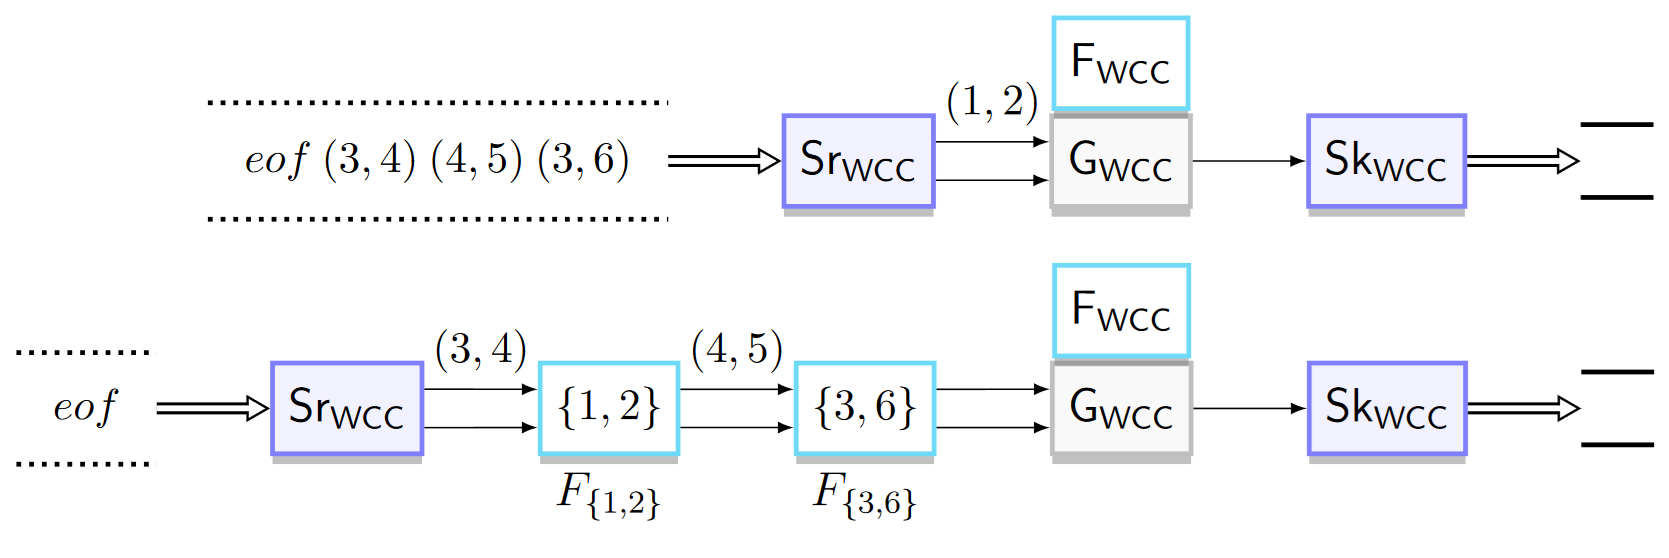
\includegraphics[width=\textwidth]{figures/ExampleBiTriangles.png}
        \caption{Dynamic Pipeline for bitriangles in bigraphs. Images from \cite{Royo_Sales_2021}}
    \end{subfigure}
    \hfill
    \begin{subfigure}{\textwidth}
    \centering
       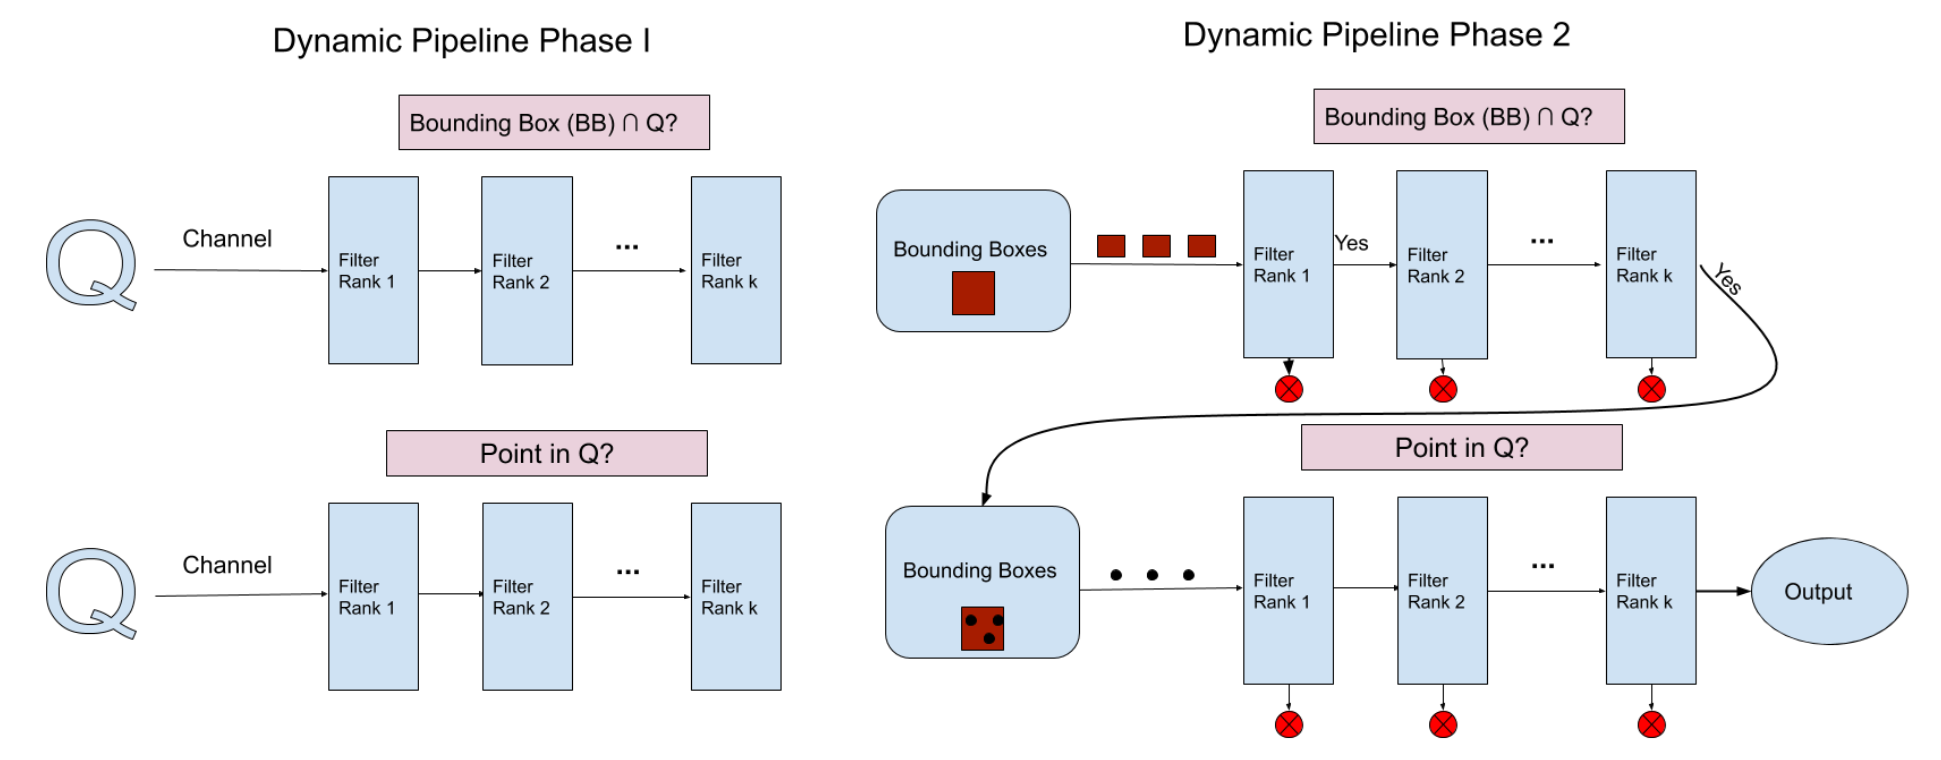
\includegraphics[width=\textwidth]{figures/ExampleQuadtree.png} 
       \caption{Dynamic Pipeline for Quadtrees. Image from \cite{Lugosi_Enes_2019}}
    \end{subfigure}
    \caption{Examples of different problems in \dpm.\label{fig:examples_dp}}
\end{figure}